\section{溶液作製精度に関して}

溶液の作製精度の確認を行うため,0.95,1.00,1.05wt.\%のPAA溶液を作製した.それぞれの擬塑性流体に直径10mmの鋼球を落下させ,終端速度の変化,超音波照射による影響の変化の確認を行った.

\subsection{溶液の粘性特性に関して}
それぞれの溶液の特性を確認するため,粘度計を用いて粘度計測を行った.粘度計測を行った結果をFig.\ref{fig:95-105}に示す.比較のため,先行研究である岩室\cite{ref:8}とShiratori \it{et al}.\cite{ref:9}の計測結果も合わせて示す.濃度が薄いと粘度は低く,濃度が高いと粘度は高くなった.

\begin{figure}[ht]
    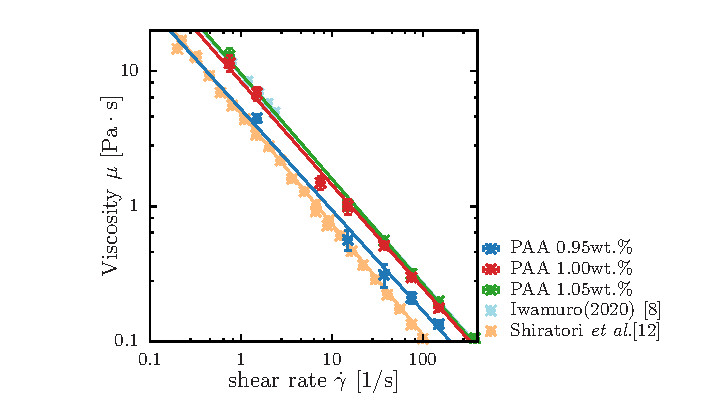
\includegraphics[width=1\textwidth]{X-Appendix/concentration/viscosity/viscosity.eps}
    \caption{Viscosity versus shear rate for PAA0.95,1.00,1.05wt.\%.}
    \label{fig:95-105}
\end{figure}

\subsection{溶液の作製精度による高速化への影響に関して}

ぞれぞれの質量濃度のPAA溶液に対し,落下球実験を行った.落下させた球は,鋼製の直径10mmの球である.

\subsection{溶液の作製精度と終端速度の関係}

実験装置の改良により終端速度に差異がみられた.終端速度の差異に関して考察を行う.式(\ref{eq:UT})より,Power-Law modelにおける,$k$,$n$のパラメータより終端速度を見積もることができる.

Table \ref{table:power-law}の結果より,式(\ref{eq:UT})を用いて直径10mmの球におけるIwamuro\cite{ref:8}の終端速度$U_I$を基準とした終端速度の比$U_T/U_{I}$を求めた.その結果を,Table \ref{table:UT}に示す.これより,今回の粘度特性において,Iwamuro\cite{ref:8}と比較して終端速度が1.09倍速くなることが分かった.Fig.\ref{fig:falling-A}において,Iwamuro\cite{ref:8}と比較して1.125倍,終端速度が速かった.一方で,0.95,1.05wt.\%それぞれのPAA溶液の粘度特性における終端速度比と比較しても実験結果と一番近いのは,1wt.\%の場合である.よって,溶液の濃度精度は1wt.\%±0.05wt.\%以内であり,溶液の作製誤差によって落下速度に差が生じたと考えられる.

\begin{table}[h]
    \centering
    \caption{Each parameter($k$,$n$) and terminal speed ratio in the power-law model for each experimental result.}
    \label{table:UT}
    \begin{tabular}{c|c|c|c} \hline
                                                     & $k$  & $n$  & $U_T/U_{I}$ \\ \hline \hline
        Present Value(1.05wt.\%)                     & 9.56 & 0.23 & 0.93        \\
        Present Value(1wt.\%)                        & 8.37 & 0.24 & 1.09        \\
        Present Value(0.95wt.\%)                     & 5.22 & 0.25 & 3.91        \\
        Iwamuro\cite{ref:8}                          & 9.4  & 0.23 & 1           \\
        Shiratori \textit{et al}.(2016)\cite{ref:10} & 5.9  & 0.25 & 2.99        \\ \hline
    \end{tabular}
\end{table}

